\documentclass[11pt,a4paper]{article}
\usepackage[margin=2.5cm]{geometry}
\usepackage[T1]{fontenc}
\usepackage[utf8]{inputenc}
\usepackage{amsmath,amsthm,amssymb}
\usepackage{graphicx}
\usepackage{booktabs}
\usepackage{tikz}
\usepackage[hidelinks]{hyperref}
\usepackage{cleveref}
\usepackage[backend=biber,style=numeric,urldate=long]{biblatex}
\addbibresource{references.bib}
\graphicspath{{figures/}}

\theoremstyle{definition}
\newtheorem{definition}{Definition}[section]
\newtheorem{example}[definition]{Example}
\newtheorem{nonexample}[definition]{Non-example}
\theoremstyle{plain}
\newtheorem{theorem}[definition]{Theorem}
\newtheorem{lemma}[definition]{Lemma}
\newtheorem{proposition}[definition]{Proposition}
\newtheorem{corollary}[definition]{Corollary}
\theoremstyle{remark}
\newtheorem{remark}[definition]{Remark}

% Opening words of every plain-words paragraph.
\newcommand{\plainwords}{\noindent\textbf{In plain words.}}


\title{Adjacency matrices, walks, and connectivity:\\
what the powers of $A$ count and how $A$ shows that a graph is connected}
\author{}
\date{\today}

\begin{document}
\maketitle

\begin{abstract}
A finite simple undirected graph with $N$ vertices can be given by its
adjacency matrix $A$. This note answers three questions about it, two
taken from a lecture whiteboard and one from an assignment. First, the
entry in row $i$ and column $j$ of the matrix power $A^k$ counts the walks
of length $k$ from vertex $n_i$ to vertex $n_j$; it counts walks, not
paths. Second, the graph is connected if and only if every entry off the
diagonal of $A+A^2+\dots+A^{N-1}$ is positive, which holds if and only if
$(I+A)^{N-1}$ has no zero entry. Third, a path between $n_i$ and $n_j$ is
a sequence of pairwise distinct vertices from $n_i$ to $n_j$ in which
consecutive vertices are adjacent, the course textbook's simple path. All
statements are proved in full, the course textbook's numbering is used for
its definitions, and every matrix in the worked examples was computed by
script. Each definition, theorem, and test is preceded by a plain-words
paragraph told as a story about a frog on islands.
\end{abstract}

\section{Introduction}\label{sec:intro}

\subsection{The question and where it came from}

A lecture whiteboard shows a small graph, its table of zeros and ones, and two questions about that table \cite{whiteboard1,whiteboard2}.
The board states the problem as follows: a graph with $N$ nodes is given through its adjacency matrix $A$; (1) what does the entry in row $i$ and column $j$ of a power of $A$ represent, and (2) how does one know whether the graph is connected \cite{whiteboard1,whiteboard2}.
The board also gives a definition of a connected graph, which uses the word ``path'' \cite{whiteboard1,whiteboard2}.
The assignment text added a third question: what is the definition of a path between two vertices $n_i$ and $n_j$.
That third question comes from the assignment, not from the board.
The paper therefore answers three questions.

\begin{enumerate}
\item[Q1.] What does the entry $(A^k)_{ij}$ of the $k$-th power of the adjacency matrix represent?
\item[Q2.] How can one decide from $A$ alone whether the graph is connected?
\item[Q3.] What is the definition of a path between the vertices $n_i$ and $n_j$?
\end{enumerate}

\emph{Reading of the board.}
In question 1 the board puts a small mark above the letter $A$.
In both photographs the mark looks like a small $n$ or a pair of quotation marks, not clearly a $k$ \cite{whiteboard1,whiteboard2}.
This paper reads the mark as an exponent $k$, because the assignment text asks about $A^k$.
This is an interpretation, and it is qualified: the board does not settle it.
It does not change the mathematics, because \cref{thm:walks} holds for every positive whole exponent, whatever letter is used.

\subsection{The story used throughout}\label{sec:story}

Every explanation marked ``In plain words'' uses one story.
A village has a number of houses.
Each house is a point.
Each road joins exactly two different houses.
Every road can be driven in both directions.
No road leads from a house back to itself.
No two roads join the same pair of houses.
A trip is a list of houses, one after another, where each house is at the other end of a road from the house before.
A trip may pass the same house twice and may drive the same road twice.
A clean route is a trip that never visits the same house twice.
The village of the board has three houses in a row: a road from the first house to the second, and a road from the second house to the third.
The first and third houses have no road between them.
The mathematics below uses the same village; the terms are matched in \cref{tab:story}.

\begin{table}[ht]
\centering
\caption{The story and the mathematics. The right column names the definitions that are introduced in \cref{sec:background}.}\label{tab:story}
\begin{tabular}{@{}ll@{}}
\toprule
Story & Mathematics\\
\midrule
house & vertex\\
road & edge\\
village & simple undirected graph (\cref{def:graph})\\
trip & walk (\cref{def:walk})\\
clean route & path (\cref{def:path})\\
table of roads & adjacency matrix (\cref{def:adjmat})\\
village in one piece & connected graph (\cref{def:connected})\\
\bottomrule
\end{tabular}
\end{table}

\subsection{What the paper shows}

The answers, stated briefly and proved later, are these.

\begin{itemize}
\item \emph{Q1} (\cref{sec:walks}). For $k\ge1$, the entry $(A^k)_{ij}$ is the number of walks of length $k$ from $n_i$ to $n_j$.
The statement appears in standard lecture notes \cite{quinlan_matrices_graphs,bai2025adjacency}; the proof in this paper is written out in full.
The entry counts walks, not paths, and \cref{prop:warning} gives a counterexample.
One web source states the theorem with the word ``paths'', which is wrong for the usual meanings of that word \cite{paramadevan2021adjacency}; this is discussed in \cref{sec:disagree}.
\item \emph{Q2} (\cref{sec:conn}). For $N\ge2$ vertices the graph is connected if and only if every entry off the diagonal of $A+A^2+\dots+A^{N-1}$ is positive.
A published note states this test and lecture notes state its second form, and both prove it loosely \cite{paramadevan2021adjacency,bai2025adjacency}.
The proof in this paper is complete (derived here).
\item \emph{Q3} (\cref{sec:pathdef}). A path between $n_i$ and $n_j$ is a walk from $n_i$ to $n_j$ with no repeated vertex.
This is the course textbook's simple path, Definition 1.2.13 \cite[p.~22]{petrosyan2015grafneri}.
\end{itemize}

The course textbook states neither the walk-counting theorem nor the matrix test in the pages that were checked, and a search of the whole book found no such theorem or test; the absence is qualified because the rest of the book was not read page by page \cite{petrosyan2015grafneri}.
Both results are therefore proved here, and the text says so each time.

\subsection{Conventions, assumptions, and kinds of statement}\label{sec:conventions}

\paragraph{Assumptions.}
The graph is finite, simple, and undirected.
This is the setting of the assignment, and it agrees with the symmetric matrix with zero diagonal on the board \cite{whiteboard1,whiteboard2}.
The textbook's graphs are of this kind too \cite[p.~9]{petrosyan2015grafneri}.
Directed graphs and graphs with repeated edges are not treated (\cref{sec:limits}).

\paragraph{The example graph.}
The board shows a drawing of three vertices and, beside it, a matrix with rows $(0\ 1\ 0)$, $(1\ 0\ 1)$, $(0\ 1\ 0)$.
The matrix encodes the two edges $n_1n_2$ and $n_2n_3$ only.
The drawing shows three lines: one from $1$ to $2$ with an arrowhead at $2$, one from $1$ to $3$, and one from $2$ to $3$ \cite{whiteboard1,whiteboard2}.
So the drawing has an edge $1$--$3$ that the matrix lacks, and an arrowhead that a symmetric matrix does not support.
The problem statement says that the graph is given through its adjacency matrix \cite{whiteboard1,whiteboard2}.
This paper therefore takes the matrix as the example graph, calls it the \emph{board graph}, and treats the extra line and the arrowhead as a mismatch that it reports and does not resolve.
When a graph with a cycle is needed, the drawing's triangle is used and is labelled as the triangle.

\paragraph{Notation.}
\Cref{tab:notation} fixes the letters.
The board writes $(G,V)$ for the graph and $e_{ij}\in V$ in its matrix definition, where its $V$ is the edge set; the textbook writes $G=(V,E)$ with $E$ the edge set \cite{whiteboard1,whiteboard2,petrosyan2015grafneri}.
This is a difference of notation only.
The board names the vertices $n_i$; the textbook names them $v_i$ \cite{whiteboard1,whiteboard2,petrosyan2015grafneri}.
This paper uses the board's $n_i$.

\begin{table}[ht]
\centering
\caption{Notation used in this paper.}\label{tab:notation}
\begin{tabular}{@{}p{0.2\textwidth}p{0.72\textwidth}@{}}
\toprule
Symbol & Meaning\\
\midrule
$G=(V,E)$ & a finite simple undirected graph with vertex set $V$ and edge set $E$ (textbook letters)\\
$N$ & the number of vertices, $N=|V|$ (the board writes $|G|=N$)\\
$n_1,\dots,n_N$ & the vertices (the board's names; the textbook's $v_i$)\\
$uv$, $e_{ij}$ & the edge between $u$ and $v$; the edge between $n_i$ and $n_j$\\
$A$, $A_{ij}$ & the adjacency matrix and its entry in row $i$, column $j$\\
$A^k$, $(A^k)_{ij}$ & the $k$-th power of $A$ and its entry in row $i$, column $j$\\
$I$ & the $N\times N$ identity matrix (ones on the diagonal, zeros elsewhere)\\
$k$ & the length of a walk, or an exponent; a positive whole number unless stated\\
$S$ & the sum $A+A^2+\dots+A^{N-1}$ (\cref{def:S})\\
$\deg(n_i)$ & the degree of $n_i$ (\cref{def:degree})\\
$d(u,v)$ & the distance between $u$ and $v$ (\cref{def:distance})\\
\bottomrule
\end{tabular}
\end{table}

\paragraph{The word ``path''.}
The word has more than one meaning in the sources.
The textbook's own ``path'' (Definition 1.2.12) allows a repeated vertex, and it calls a path without a repeated vertex a ``simple path'' (Definition 1.2.13) \cite[p.~22]{petrosyan2015grafneri}.
Two English texts call the second kind a path and the first kind a trail \cite{grinberg2025graph,wikipedia_path_graph_theory}.
The assignment states that in the course a path has no repeated vertex; that statement comes from the assignment text and not from a file, so it is recorded as an interpretation.
This paper uses \emph{path} for a walk without repeated vertices and \emph{trail} for the textbook's Definition 1.2.12, and \cref{tab:naming} gives the three conventions side by side.

\paragraph{Kinds of statement.}
A statement with a citation is taken from the cited source.
A statement marked \emph{derived} is proved or computed in this paper; every number in such a statement was computed by script (\cref{app:repro}).
Statements marked \emph{interpretation}, \emph{estimate}, or \emph{open} are labelled in the same way, and the textbook's definition numbers are always written ``textbook Definition~1.2.10'' and so on, so that they cannot be mistaken for the numbers of this paper.

\subsection{Organization}

\Cref{sec:background} builds the prerequisites in the textbook's order: graph, adjacency, the adjacency matrix, walk, trail, path, cycle, and distance, with the lemma that every walk contains a path.
\Cref{sec:walks} answers Q1, \cref{sec:conn} answers Q2, and \cref{sec:pathdef} answers Q3.
\Cref{sec:examples} works the board graph and three further graphs through in full.
\Cref{sec:discussion} states the limits, and \cref{sec:conclusion} gives the direct answers.
The appendices hold longer derivations, the textbook's terms, the transcription of the photographs, and the scripts.

\section{Graphs and the adjacency matrix}\label{sec:background}

\paragraph{Notation.} Throughout, $G=(V,E)$ is a finite simple undirected
graph (Convention~\ref{conv:setting}) with vertex set
$V=\{n_1,\dots,n_N\}$, $N\ge 1$, and edge set $E$. The letters $u,v,w$
also stand for vertices; $uv$ is the edge joining $u$ and $v$, and
$|E|$ is the number of edges. The indices $i,j,r$ run over $1,\dots,N$.
The letter $k$ is a non-negative integer used for the length of a walk and
for the exponent of a matrix power. $A$ is the adjacency matrix, $I$ the
$N\times N$ identity matrix, and $\deg(n_i)$ the degree of $n_i$. The textbook
writes the same objects with $v_i$ and $d_G(v)$
\cite[pp.~9, 16]{petrosyan2015graphs}; this note writes $\deg$ for degree so
that the letter $d$ is free for distance (\cref{def:distance}).

\subsection{Graphs, neighbours, and the adjacency matrix}

\plainwords{} A pond has some islands. Some pairs of islands have a bridge
between them. A bridge joins two different islands. No two islands have
more than one bridge. A bridge can be crossed in both directions.

\begin{definition}[Graph; textbook Definition~1.1.1]\label{def:graph}
A \emph{graph} $G$ is an ordered pair $(V,E)$, where $V$ is a set whose
elements are the \emph{vertices} and $E$ is a set whose elements are the
\emph{edges} \cite[Definition~1.1.1, p.~9]{petrosyan2015graphs}. In this
note $V$ is finite, and each edge is a set $uv=\{u,v\}$ of two different
vertices (Convention~\ref{conv:setting}).
\end{definition}

\begin{remark}
Because an edge is a set of two different vertices, there is no edge from
a vertex to itself, and $uv$ and $vu$ are the same edge, so there is no
direction. Because $E$ is a set, two vertices are joined by at most one
edge.
\end{remark}
\begin{example}
The board graph has $V=\{n_1,n_2,n_3\}$ and $E=\{n_1n_2,\,n_2n_3\}$
(\cref{fig:graphs}, left).
\end{example}
\begin{nonexample}
Giving $n_1$ an edge to itself, or giving $n_1$ and $n_2$ two separate
edges, does not produce a graph in this note's sense.
\end{nonexample}

\plainwords{} Two islands are next door when one bridge joins them. If a
frog can hop between two islands in one hop, they are next door. An island
is never next door to itself.

\begin{definition}[Adjacent; textbook Definition~1.1.4]\label{def:adjacent}
The vertices $u$ and $v$ are \emph{adjacent} if $uv\in E$
\cite[Definition~1.1.4, p.~11]{petrosyan2015graphs}.
\end{definition}

\begin{remark}
Adjacency is symmetric, and in a simple graph no vertex is adjacent to
itself.
\end{remark}
\begin{example}
In the board graph, $n_1$ and $n_2$ are adjacent.
\end{example}
\begin{nonexample}
In the board graph, $n_1$ and $n_3$ are not adjacent, and neither is
$n_2$ with itself.
\end{nonexample}

\plainwords{} Draw a square table. Give each island one row and one
column. Put a one in a cell when the row island and the column island are
next door. Put a zero in every other cell. The table lists all the
bridges.

\begin{definition}[Adjacency matrix; textbook, after Definition~1.1.6]\label{def:matrix}
The \emph{adjacency matrix} of $G$ is the $N\times N$ matrix $A=(A_{ij})$
with
\begin{equation}\label{eq:adj}
A_{ij}=\begin{cases}1,& n_i \text{ and } n_j \text{ are adjacent},\\
0,& \text{otherwise.}\end{cases}
\end{equation}
The textbook gives this matrix no number of its own; it states the rule
and notes $a_{ii}=0$ and $a_{ij}=a_{ji}$ on printed p.~11
\cite{petrosyan2015graphs}. The board writes the same rule as $A_{ij}=1$
if $e_{ij}\in V$ and $0$ if $e_{ij}\notin V$, with $e_{ij}$ the edge
joining $n_i$ and $n_j$ and $V$ the board's name for the edge set
\cite{whiteboard1,whiteboard2} (Convention~\ref{conv:names}).
\end{definition}

\begin{remark}
Every entry is $0$ or $1$, never $2$ or a weight, which is correct because
a simple graph has at most one edge between two vertices. A $1$ on the
diagonal would be a loop, which a simple graph does not have.
\end{remark}
\begin{example}
The board matrix has rows $0\,1\,0$, $1\,0\,1$, $0\,1\,0$
\cite{whiteboard1,whiteboard2}:
\[
A=\begin{pmatrix}0&1&0\\1&0&1\\0&1&0\end{pmatrix}.
\]
It is the adjacency matrix of the board graph, whose only edges are
$n_1n_2$ and $n_2n_3$ (Convention~\ref{conv:drawing}).
\end{example}
\begin{nonexample}
The matrix with rows $0\,1\,0$, $0\,0\,1$, $0\,1\,0$ is not the adjacency
matrix of a simple undirected graph, because it is not symmetric. A matrix
with a $1$ in the top left corner is not one either, because that $1$ would
be a loop.
\end{nonexample}

\plainwords{} Count the bridges that touch one island. That count is the
number of bridges at the island.

\begin{definition}[Degree; textbook Definition~1.2.1]\label{def:degree}
The \emph{degree} $\deg(n_i)$ of the vertex $n_i$ is the number of edges that
have $n_i$ as an end \cite[Definition~1.2.1, p.~16]{petrosyan2015graphs}.
\end{definition}

\begin{remark}
The textbook defines degree after the adjacency matrix, so this note uses
it only after \cref{def:matrix}.
\end{remark}
\begin{example}
In the board graph the degrees of $n_1,n_2,n_3$ are $1,2,1$.
\end{example}
\begin{nonexample}
The number of edges of the board graph, which is $2$, is not the degree of
$n_1$, which is $1$.
\end{nonexample}

\plainwords{} Flip the table over its slanted line of cells from top left
to bottom right. Nothing changes. Cells on that line stay zero, because no
island is next door to itself. Add up one row. You get the number of
bridges at that island. Add up the whole table. You count every bridge
twice.

\begin{proposition}[Basic properties of $A$]\label{prop:basic}
Let $A$ be the adjacency matrix of $G$. Then
\begin{enumerate}
\item $A_{ij}=A_{ji}$ for all $i,j$ (symmetry);
\item $A_{ii}=0$ for all $i$ (zero diagonal);
\item $\sum_{j}A_{ij}=\deg(n_i)$ for every $i$ (row sums are degrees);
\item $\sum_{i,j}A_{ij}=2|E|$.
\end{enumerate}
\end{proposition}
Items 1 and 2 are stated in the textbook \cite[p.~11]{petrosyan2015graphs}
and in the University of Galway notes \cite[Notes~1 and 2, p.~3]{galwaynotes};
the proof below is the note's own.
\begin{proof}
(1) $n_i$ and $n_j$ are adjacent exactly when $n_j$ and $n_i$ are, since
$uv=vu$. (2) A simple graph has no edge from $n_i$ to itself, so $n_i$ is
not adjacent to itself. (3) Row $i$ has a $1$ in column $j$ exactly when
$n_in_j\in E$, so the row sum counts the edges at $n_i$, which is
$\deg(n_i)$. (4) By (3) the sum of all entries is the sum of all degrees. Every edge has
two ends, so it is counted once at each end when the degrees are added; the
sum is therefore $2|E|$, which is the textbook's Theorem~1.2.1 (Euler)
\cite[Theorem~1.2.1, p.~16]{petrosyan2015graphs}. Since $A$ is symmetric,
column sums are the degrees too.
\end{proof}

\subsection{Matrix products and powers}

\plainwords{} To make a new table from two tables, take one row of the
first and one column of the second. Multiply their cells in pairs. Add the
results. That is one cell of the new table. Do this for every row and
column. Do it to the island table with itself, and again, and again.

\begin{definition}[Matrix product and power]\label{def:power}
For $N\times N$ matrices $X$ and $Y$ the product $XY$ has entries
\begin{equation}\label{eq:product}
(XY)_{ij}=\sum_{r=1}^{N}X_{ir}Y_{rj}.
\end{equation}
The \emph{powers} of $A$ are $A^0=I$ (ones on the diagonal, zeros
elsewhere) and $A^{k+1}=A^{k}A$ for $k\ge 0$. This is the standard
definition from linear algebra. In words, the entry in row $i$ and column
$j$ of $XY$ is obtained by running along row $i$ of $X$ and down column $j$
of $Y$, multiplying the entries in pairs, and adding the results. The
\emph{transpose} $X^{T}$ of $X$ is the matrix with $(X^{T})_{ij}=X_{ji}$,
that is, $X$ flipped over its diagonal; the standard rule
$(XY)^{T}=Y^{T}X^{T}$ is used in \cref{sec:counting}. By
\cref{prop:basic}, $A^{T}=A$.
\end{definition}

\begin{remark}\label{rem:nonneg}
A power is not the entrywise power. Every entry of $A^k$ is a non-negative
integer, because $A$ has entries $0$ and $1$ and sums and products of
non-negative integers are non-negative integers; this is used in
\cref{sec:connectivity}.
\end{remark}
\begin{example}
For the board matrix, row $1$ of $A$ is $(0,1,0)$ and column $1$ of $A$ is
$(0,1,0)$, so $(A^2)_{11}=0\cdot 0+1\cdot 1+0\cdot 0=1$. Row $2$ is
$(1,0,1)$ and column $2$ is $(1,0,1)$, so
$(A^2)_{22}=1\cdot 1+0\cdot 0+1\cdot 1=2$.
\end{example}
\begin{nonexample}
Squaring every entry of $A$ separately gives $A$ back, because the entries
are $0$ or $1$; it is not $A^2$, whose entry in row $2$ and column $2$ is
$2$, not $0$.
\end{nonexample}

\section{Walks, trails, paths, and cycles}\label{sec:walks}

This section answers question (Q3), the definition of a path between $n_i$
and $n_j$, in the order in which the textbook builds the concepts
\cite[pp.~21--23]{petrosyan2015graphs}: walk, closed walk, trail, path,
cycle, distance. Each concept is a small change to the one before it. The
examples use the graph $H$ on five vertices with edges $n_1n_2$, $n_2n_3$,
$n_1n_3$, $n_3n_4$, $n_4n_5$ (\cref{fig:graphs}, middle), which is this
note's own example, not the textbook's; the classification of every
sequence below was checked by script (\cref{app:repro}).

Only walks and paths (\cref{def:walk,def:path,def:pathbetween}) and the
lemmas on them are needed for (Q1) to (Q3). Trails are included because the
textbook uses the word ``path'' for them and its definition of connected
rests on that word; cycles and distance are included to keep the textbook's
order, and distance is used in \cref{cor:dist}.

\begin{figure}[ht]
\centering
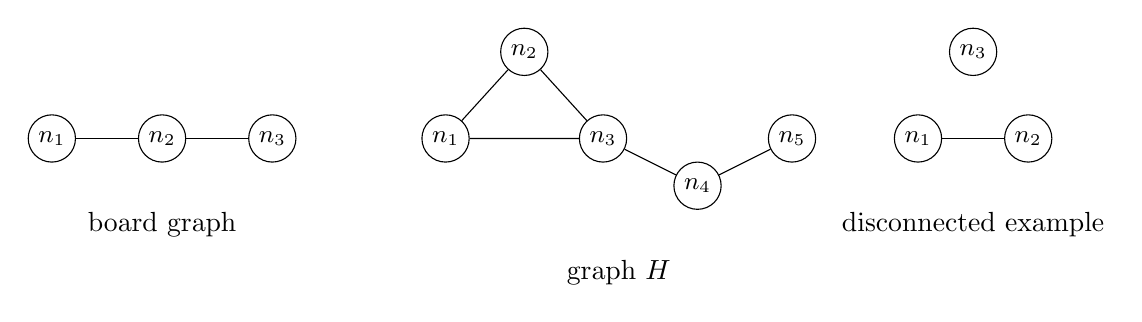
\begin{tikzpicture}[v/.style={circle,draw,inner sep=1.2pt,minimum size=6mm,font=\small},scale=1]
% board graph
\begin{scope}
\node[v] (a1) at (0,0) {$n_1$};
\node[v] (a2) at (1.4,0) {$n_2$};
\node[v] (a3) at (2.8,0) {$n_3$};
\draw (a1)--(a2)--(a3);
\node at (1.4,-1.1) {board graph};
\end{scope}
% graph H
\begin{scope}[xshift=5cm]
\node[v] (b1) at (0,0) {$n_1$};
\node[v] (b2) at (1,1.1) {$n_2$};
\node[v] (b3) at (2,0) {$n_3$};
\node[v] (b4) at (3.2,-0.6) {$n_4$};
\node[v] (b5) at (4.4,0) {$n_5$};
\draw (b1)--(b2)--(b3)--(b1);
\draw (b3)--(b4)--(b5);
\node at (2.2,-1.7) {graph $H$};
\end{scope}
% disconnected example
\begin{scope}[xshift=11cm]
\node[v] (c1) at (0,0) {$n_1$};
\node[v] (c2) at (1.4,0) {$n_2$};
\node[v] (c3) at (0.7,1.1) {$n_3$};
\draw (c1)--(c2);
\node at (0.7,-1.1) {disconnected example};
\end{scope}
\end{tikzpicture}
\caption{The graphs used in the examples. Left: the board graph, with
edges $n_1n_2$ and $n_2n_3$ and the adjacency matrix of the board
(Convention~\ref{conv:drawing}). Middle: the graph $H$ of this section, with edges $n_1n_2$, $n_2n_3$,
$n_1n_3$, $n_3n_4$, $n_4n_5$.
Right: one edge and an isolated vertex, the disconnected example of
\cref{sec:connectivity}.}\label{fig:graphs}
\end{figure}

\paragraph{Notation.} A \emph{$(u,v)$-walk} is a walk from $u$ to $v$.
In examples, a sequence of vertices such as $n_1n_2n_3$ is written
without commas.

\subsection{The definitions}

\plainwords{} A frog sits on an island. It hops over a bridge to a
next-door island, then hops again. The list of islands it visits is a
trip. A trip may land on an island again. It may use a bridge again. The
number of hops is how long the trip is. A frog that does not hop at all
makes a trip with no hops.

\begin{definition}[Walk; textbook Definition~1.2.10]\label{def:walk}
A \emph{walk from $u_0$ to $u_k$} is a sequence of vertices
$u_0u_1\cdots u_k$ in which each vertex is adjacent to the one before it;
its \emph{length} is $k$, the number of edges used. Formally, the textbook
defines it as a sequence $u_0,e_1,u_1,\dots,e_k,u_k$ of vertices and edges
with $e_t=u_{t-1}u_t$ for $1\le t\le k$
\cite[Definition~1.2.10, p.~21]{petrosyan2015graphs}; in a simple graph the
edges are fixed by the vertices, so the vertex sequence says the same. This
note allows $k=0$ (Convention~\ref{conv:length}), which the textbook's
definition does not state in words.
\end{definition}

\begin{remark}
Vertices and edges may repeat, and the length counts each edge as often as
it is used \cite[p.~22]{petrosyan2015graphs}. A single vertex $u$ is a walk
of length 0 from $u$ to $u$ (Convention~\ref{conv:length}).
\end{remark}
\begin{example}
In $H$, the sequence $n_1n_2n_3n_4n_3n_1$ is a walk of length $5$.
\end{example}
\begin{nonexample}
In $H$, the sequence $n_1n_4$ is not a walk, because $n_1n_4$ is not an
edge.
\end{nonexample}

\plainwords{} A round trip ends on the island where it began.

\begin{definition}[Closed walk; textbook Definition~1.2.11]\label{def:closed}
A walk $u_0\cdots u_k$ is \emph{closed} if $u_0=u_k$
\cite[Definition~1.2.11, p.~22]{petrosyan2015graphs}.
\end{definition}

\begin{remark}
A walk of length 0 is closed, and so is a walk that goes along one edge
and straight back.
\end{remark}
\begin{example}
In $H$, the walk $n_1n_2n_1$ is closed.
\end{example}
\begin{nonexample}
In $H$, the walk $n_1n_2n_3$ is not closed.
\end{nonexample}

\plainwords{} A fresh-bridge trip never uses the same bridge twice. It may
land on an island again.

\begin{definition}[Trail; textbook Definition~1.2.12, where it is called ``path'']\label{def:trail}
A walk is a \emph{trail} if its edges $u_0u_1,\dots,u_{k-1}u_k$ are
pairwise distinct. Its length is its number of edges
\cite[Definition~1.2.12, p.~22]{petrosyan2015graphs}.
\end{definition}

\begin{remark}
The textbook's word for a trail is ``path'' (Convention~\ref{conv:path}),
which is not what this note means by ``path''. In a trail vertices may
repeat but edges may not. The English word ``trail'' for this notion is
used by Grinberg \cite[Definition~3.4.5, p.~101]{grinberg2025graph}; it is
this note's choice for the textbook's concept, because the course's word
for it was not reported.
\end{remark}
\begin{example}
In $H$, the walk $n_3n_1n_2n_3n_4$ is a trail: its edges $n_3n_1$,
$n_1n_2$, $n_2n_3$, $n_3n_4$ are distinct, although $n_3$ occurs twice.
\end{example}
\begin{nonexample}
In $H$, the walk $n_1n_2n_1n_3$ is not a trail, because it uses the edge
$n_1n_2$ twice.
\end{nonexample}

\plainwords{} A fresh-island trip never lands on the same island twice.

\begin{definition}[Path; textbook Definition~1.2.13, the ``simple path'']\label{def:path}
A walk is a \emph{path} if its vertices $u_0,\dots,u_k$ are pairwise
distinct. This is the textbook's simple path, defined there as a
textbook ``path'' (a trail) with distinct vertices
\cite[Definition~1.2.13, p.~22]{petrosyan2015graphs}; it is the course
convention (Convention~\ref{conv:path}).
\end{definition}

\begin{remark}
Every path is a trail, because distinct vertices force distinct edges
(\cref{lem:distinct}); every trail is a walk; the converses fail. This is
why the definition here needs only ``no repeated vertex'', whereas the
textbook states it as a trail with distinct vertices.
\end{remark}
\begin{example}
In $H$, the walk $n_1n_3n_4n_5$ is a path of length $3$, and so is
$n_1n_2n_3n_4n_5$, of length $4$.
\end{example}
\begin{nonexample}
In $H$, the trail $n_3n_1n_2n_3n_4$ is not a path, because $n_3$ occurs
twice. The walk $n_1n_2n_1$ is not a path either.
\end{nonexample}

\plainwords{} Pick two islands. Sometimes the frog can get from the first to the
second. If it lands on no island twice, that is a fresh-island trip between
them. A frog that stays put makes such a trip from an island to itself.

\begin{definition}[Path between $n_i$ and $n_j$; the answer to (Q3)]\label{def:pathbetween}
Let $n_i,n_j\in V$. A \emph{path between $n_i$ and $n_j$} (also a path
\emph{from $n_i$ to $n_j$}) is a sequence $u_0,u_1,\dots,u_k$ with
$k\ge 0$, $u_0=n_i$, $u_k=n_j$, such that $u_{t-1}$ and $u_t$ are adjacent
for $1\le t\le k$ and $u_0,\dots,u_k$ are pairwise distinct. Its length is
$k$. This is \cref{def:path} with the ends fixed, that is, the
textbook's Definition~1.2.13 with ends $n_i$ and $n_j$.
\end{definition}

\begin{remark}
If $i\ne j$, such a path has at least one edge. If $i=j$, the only path is
the single vertex $(n_i)$ of length 0, because $u_0=u_k$ with $k\ge 1$
would repeat a vertex. Two vertices may be joined by several paths of
different lengths.
\end{remark}
\begin{example}
In the board graph the only path from $n_1$ to $n_3$ is $n_1n_2n_3$, of
length $2$. In $H$ there are two paths from $n_1$ to $n_4$: $n_1n_3n_4$
and $n_1n_2n_3n_4$.
\end{example}
\begin{nonexample}
In the board graph, $n_1n_2n_1n_2n_3$ is a walk from $n_1$ to $n_3$ but not
a path, because it repeats $n_1$. And $n_1n_2n_1$ is not a path from $n_1$
to $n_1$.
\end{nonexample}

\plainwords{} Some round trips never use a bridge twice. If such a round trip
also lands twice on no island except the first, we call it a ring trip. A
ring trip needs at least three bridges.

\begin{definition}[Closed trail and cycle; textbook Definitions 1.2.14 and 1.2.15]\label{def:cycle}
A \emph{closed trail} is a closed walk that is a trail. The textbook calls
it a ``closed path or cycle'' \cite[Definition~1.2.14,
p.~22]{petrosyan2015graphs}. A \emph{cycle} is a closed trail of positive
length whose only repeated vertices are its first and last; this is the
textbook's simple cycle \cite[Definition~1.2.15, p.~22]{petrosyan2015graphs}
and the English ``cycle''. The word ``cycle'' is used only in this sense.
\end{definition}

\begin{remark}
In a simple graph a cycle has length at least $3$. Length $1$ would need an
edge from a vertex to itself. Length $2$ would be $w_0w_1w_0$, which uses
the edge $w_0w_1$ twice and is not a trail. The textbook's $C_n$ has
$n\ge 3$ \cite[p.~22]{petrosyan2015graphs}. A closed trail need not be a
cycle: in the graph with edges $n_1n_2$, $n_2n_3$, $n_1n_3$, $n_1n_4$,
$n_4n_5$, $n_1n_5$ (two triangles sharing $n_1$), the sequence
$n_1n_2n_3n_1n_4n_5n_1$ is a closed trail of length $6$ that repeats $n_1$
in the middle.
\end{remark}
\begin{example}
In $H$, the walk $n_1n_2n_3n_1$ is a cycle of length $3$.
\end{example}
\begin{nonexample}
In $H$, the walk $n_1n_2n_1$ is a closed walk but not a closed trail. The
board graph has no cycle at all.
\end{nonexample}

\plainwords{} The fewest hops between two islands is how far apart they
are. If the frog can never get from one to the other, we say they are
infinitely far apart.

\begin{definition}[Distance; textbook Definition~1.2.16]\label{def:distance}
The \emph{distance} $d(u,v)$ is the length of a shortest $(u,v)$-trail if
there is one, and $\infty$ otherwise
\cite[Definition~1.2.16, pp.~22--23]{petrosyan2015graphs}. (The textbook
words this with its own ``path'', that is, trail.)
\end{definition}

\begin{remark}
The textbook measures distance by shortest trails. \Cref{prop:distance}
shows that shortest walks and shortest paths give the same number, so this
note may say ``shortest path'' without changing the textbook's value.
\end{remark}
\begin{example}
In the board graph, $d(n_1,n_3)=2$ and $d(n_1,n_1)=0$.
\end{example}
\begin{nonexample}
Add an isolated vertex $n_4$ to the board graph. Then $d(n_1,n_4)=\infty$,
not $0$ or $3$.
\end{nonexample}

\begin{table}[ht]
\centering
\begin{tabular}{@{}p{3.6cm}p{2.5cm}p{3.4cm}p{2.2cm}p{1.5cm}@{}}
\toprule
Concept & This note (course) & Textbook's word & English & Textbook number \\
\midrule
walk, length $k\ge 0$ & walk & walk & walk & 1.2.10 \\
walk with first vertex equal to last & closed walk & closed walk & closed walk & 1.2.11 \\
walk with no repeated edge & trail & ``path'' & trail & 1.2.12 \\
walk with no repeated vertex & path & ``simple path'' & path & 1.2.13 \\
closed trail & closed trail & ``closed path or cycle'' & closed trail & 1.2.14 \\
closed trail, only first and last vertex repeat & cycle & ``simple cycle'' & cycle & 1.2.15 \\
least length of such a walk & distance & distance & distance & 1.2.16 \\
\bottomrule
\end{tabular}
\caption{Three naming conventions for the same concepts. The textbook
column is from \cite[pp.~21--23]{petrosyan2015graphs}. The English column
is the usage of Grinberg \cite[Definitions~2.9.1(c), 2.10.1(b),
3.4.5]{grinberg2025graph} and of Bai, who defines a path as a walk where no
vertex is repeated \cite[p.~1]{bai2025adjacency}; it is the usage of those
two sources, not a survey of English books. The word ``trail'' in the
middle column is this note's choice (Convention~\ref{conv:path}).}\label{tab:naming}
\end{table}

\subsection{Results about walks and paths}

\plainwords{} A fresh-island trip never lands on an island twice. So it
cannot use the same bridge twice either.

\begin{lemma}[Distinct vertices give distinct edges]\label{lem:distinct}
A walk $u_0\cdots u_k$ whose vertices are pairwise distinct has pairwise
distinct edges. Hence every path is a trail.
\end{lemma}
The textbook's Definition~1.2.13 asks for both properties
\cite[p.~22]{petrosyan2015graphs}; the proof is the note's own.
\begin{proof}
Suppose two edges are equal, $e_s=e_t$ with positions $1\le s<t\le k$,
where $e_s=\{u_{s-1},u_s\}$ and $e_t=\{u_{t-1},u_t\}$. The vertex $u_{s-1}$
is an end of $e_s$, hence an end of $e_t$, so $u_{s-1}=u_{t-1}$ or
$u_{s-1}=u_t$. Because the vertices of the walk are pairwise distinct, two
of them are equal only if they have the same position, so $s-1=t-1$ or
$s-1=t$. Both are impossible, because $s<t$. So no two edges are equal.
\end{proof}

\plainwords{} Take any trip from one island to another. Suppose the frog
lands on some island twice. Cut out all the hops between the two visits.
What is left is still a trip between the same two islands. It has fewer
hops. Keep cutting. In the end the frog lands on no island twice.

\begin{lemma}[Every walk contains a path]\label{lem:cut}
Let $W=u_0\cdots u_k$ be a walk from $u$ to $v$ (equal or not). Then there
is a path from $u$ to $v$ of length at most $k$ whose edges are edges of
$W$.
\end{lemma}
The textbook's Lemma~1.2.1 states this for $u\ne v$, without a bound on
the length, and proves it by induction on the length of the walk
\cite[Lemma~1.2.1, p.~23]{petrosyan2015graphs}. Grinberg's
Corollary~2.9.7 covers $u=v$ and gives the bound
\cite[p.~39]{grinberg2025graph}. The proof below, which allows $k=0$, is the
note's own.
\begin{proof}
By strong induction on $k$: to prove the statement for walks of length $k$,
we may assume it for all shorter walks, of every length from $0$ to
$k-1$. (Ordinary induction would assume it only for length $k-1$; we need
more, because the cut below removes an unknown number of edges.)
\emph{Base case $k=0$.} Then $W=(u)$ has one vertex, which is not repeated,
so $W$ is itself a path of length $0$.
\emph{Inductive case.} Let $k\ge 1$ and assume the statement for all walks
shorter than $k$. If the vertices of $W$ are pairwise distinct, $W$ is a
path of length $k$. Otherwise there are positions $s<t$ with $u_s=u_t$,
the same vertex visited twice. Form $W'=u_0\cdots u_su_{t+1}\cdots u_k$,
that is, delete the part of $W$ between the two visits (if $t=k$, then
$W'=u_0\cdots u_s$). It is a walk, because the only new consecutive pair is
$u_s,u_{t+1}$ and $u_s=u_t$ is adjacent to $u_{t+1}$. It runs from $u$ to
$v$, its edges are edges of $W$, and its length is $k-(t-s)<k$. By the
induction hypothesis $W'$ contains a path from $u$ to $v$ of length at most
$k-(t-s)\le k$. (The example after this proof shows the cut.)
\end{proof}

\begin{example}
In the board graph, cutting the walk $n_1n_2n_1n_2n_3$ at the repeated
vertex $n_1$ leaves the path $n_1n_2n_3$; cutting the closed walk
$n_1n_2n_3n_2n_1$ leaves the path $n_1$ of length $0$.
\end{example}

\plainwords{} A fresh-island trip lands on each island at most once. So it
cannot have as many hops as there are islands. With three islands, it has
at most two hops.

\begin{corollary}[Length bound]\label{cor:bound}
A path in a graph with $N$ vertices has length at most $N-1$. Hence if
some walk joins $u$ to $v$, a path of length at most $N-1$ joins them.
\end{corollary}
\begin{proof}
A path of length $k$ has $k+1$ pairwise distinct vertices among the $N$
vertices of the graph, so $k+1\le N$ \cite[Section~2.9.4,
p.~40]{grinberg2025graph}. The second sentence follows with
\cref{lem:cut}: a walk of any length contains a path, and every path has
length at most $N-1$.
\end{proof}
The bound is attained: the path graph on $N$ vertices has a path of length
$N-1$.

\plainwords{} Suppose some trip joins two islands. Then a fresh-bridge trip
joins them, and a fresh-island trip joins them too. So it does not matter
which kind of trip we ask for.

\begin{proposition}[Walk, trail, and path exist together]\label{prop:together}
For vertices $u$ and $v$ the following are equivalent: (a) a $(u,v)$-walk
exists; (b) a $(u,v)$-trail exists; (c) a $(u,v)$-path exists.
\end{proposition}
Grinberg's Proposition~2.9.10 states the equivalence of walks and paths
only \cite[p.~42]{grinberg2025graph}; the trail case is proved here.
\begin{proof}
(c) implies (b) by \cref{lem:distinct}. (b) implies (a), because a trail
is a walk. (a) implies (c) by \cref{lem:cut}.
\end{proof}
Consequently the textbook's definition of a connected graph, which asks
for a textbook ``path'' (a trail), the board's definition, read with the
course's path, and a definition by walks select the same graphs
(\cref{sec:connectivity}).

\plainwords{} The fewest hops over all trips between two islands is the
same as the fewest hops over all fresh-bridge trips. It is also the same as
the fewest hops over all fresh-island trips.

\begin{proposition}[Distance]\label{prop:distance}
For vertices $u$ and $v$ let $L_w$, $L_t$, $L_p$ be the least length of a
walk, a trail, and a path from $u$ to $v$ (with $\infty$ if none exists).
Then $L_w=L_t=L_p=d(u,v)$.
\end{proposition}
The textbook lists three properties of distance without proof
\cite[p.~23]{petrosyan2015graphs}; the statement here and its proof are the
note's own.
\begin{proof}
Every path is a trail and every trail is a walk (\cref{lem:distinct}), so
$L_w\le L_t\le L_p$. If a walk $W$ of least length $L_w$ exists and
repeated a vertex, the cut in the proof of \cref{lem:cut} would give a
shorter walk, contradicting minimality; so $W$ is a path and
$L_p\le L_w$. The three numbers agree. The textbook's $d(u,v)$ is $L_t$ by
\cref{def:distance}. If no walk exists, all three are $\infty$.
\end{proof}

\begin{remark}
The textbook's three properties of distance then follow from walks
\cite[p.~23]{petrosyan2015graphs}. First, $d(u,v)=0$ exactly when $u=v$,
because a walk of length $0$ ends where it starts (this uses
Convention~\ref{conv:length}). Second, $d(u,v)=d(v,u)$, because reversing a
walk gives a walk of the same length. Third,
$d(u,v)\le d(u,w)+d(w,v)$, because a walk from $u$ to $w$ followed by a
walk from $w$ to $v$ is a walk from $u$ to $v$ whose length is the sum
(trivially true when a distance is $\infty$).
\end{remark}

\section{Question 1: what the entries of a power of $A$ count}\label{sec:counting}

\subsection{Matrix powers}

\plain To combine the road table with itself, pick a middle town. Ask
whether the first town is a neighbour of the middle town. Ask whether the
middle town is a neighbour of the last. Do this for every possible middle town
and add up the answers.

\begin{definition}[matrix product and power]\label{def:power}
For $N\times N$ matrices $X$ and $Y$, the product $XY$ is the $N\times N$
matrix with
\begin{equation}\label{eq:product}
(XY)_{ij}=\sum_{t=1}^{N}X_{it}Y_{tj}.
\end{equation}
The identity matrix $I$ has $I_{ii}=1$ and $I_{ij}=0$ for $i\ne j$, and
$XI=IX=X$. The powers of $A$ are $A^0=I$ and $A^{k+1}=A^kA$ for $k\ge0$.
\end{definition}

\begin{remark}
Each entry of a product is a sum over a middle index $t$. Since $A$ has only
the entries $0$ and $1$, every entry of every power of $A$ is a non-negative
integer. The exponent $k$ counts how many copies of $A$ are multiplied;
$A^0=I$ is the case of no copies.
\end{remark}

\ex For the board matrix, $(A^2)_{22}=A_{21}A_{12}+A_{22}A_{22}+A_{23}A_{32}
=1\cdot1+0\cdot0+1\cdot1=2$.
\nonex $(A^2)_{22}$ is not $A_{22}\cdot A_{22}=0$. Squaring the matrix is not
squaring each entry.

\subsection{Basic properties of $A$}

\plain The road table has a few simple habits. A town is never its own
neighbour. If one town is a neighbour of another, the second is a neighbour of
the first. Adding along a row tells how many roads leave that town.

\begin{proposition}[properties of $A$ and its powers]\label{prop:properties}
Let $A$ be the adjacency matrix of a simple graph.
\begin{enumerate}
\item[(1)] $A_{ii}=0$ and $A_{ij}=A_{ji}$ for all $i,j$
  \cite[p.~11]{petrosyan2015grafneri}.
\item[(2)] Every power of $A$ is symmetric: $(A^k)_{ij}=(A^k)_{ji}$.
\item[(3)] The $i$-th row sum of $A$ is the degree: $\sum_{j}A_{ij}=d(n_i)$.
  The column sums are equal to the row sums.
\item[(4)] $(A^2)_{ii}=d(n_i)$.
\end{enumerate}
\end{proposition}

\begin{proof}
(1) is the textbook's remark after the definition of $A(G)$, restated in
\cref{def:matrix}. (2) Using $(XY)^{T}=Y^{T}X^{T}$ repeatedly and $A^{T}=A$,
we get $(A^k)^{T}=(A^{T})^k=A^k$. (3) The sum $\sum_jA_{ij}$ counts the
vertices adjacent to $n_i$. In a simple graph these correspond one to one to
the edges at $n_i$, so the sum is $d(n_i)$ by \cref{def:degree}; by (1) the
column sums are the same. (4) By \eqref{eq:product} and (1),
$(A^2)_{ii}=\sum_tA_{it}A_{ti}=\sum_tA_{it}^2=\sum_tA_{it}=d(n_i)$,
because $A_{it}\in\{0,1\}$ gives $A_{it}^2=A_{it}$.
\end{proof}

Paramadevan and Sotheeswaran state (4) in the proof of their Theorem~1
\cite[p.~17]{paramadevan2021properties}. The textbook states (1) and does not
state (2) to (4), so those are ours. On the board matrix the row sums are
$1,2,1$, which are the degrees of \cref{def:degree}'s example.

\subsection{The walk-counting theorem}

\plain Multiply the road table by itself a few times. Each number in the
result tells how many trips of exactly that many roads lead from one town to
another. Trips may come back to a town they visited. Trips may use a road
again. Every such trip is counted.

\begin{theorem}[walk counting]\label{thm:count}
Let $G$ be a simple undirected graph with vertices $n_1,\dots,n_N$ and
adjacency matrix $A$. For every integer $k\ge0$ and all $i,j\in\{1,\dots,N\}$,
the entry $(A^k)_{ij}$ equals the number of walks of length $k$ from $n_i$
to $n_j$.
\end{theorem}

Grinberg proves the corresponding theorem for multidigraphs, which includes
$k=0$ \cite[Theorem 4.5.10, pp.~120--123]{grinberg2025introduction}. The
textbook has no such theorem (\cref{sec:sources}). The proof below is ours
and is written for simple graphs.

\begin{proof}
Write $W_k(i,j)$ for the number of walks of length $k$ from $n_i$ to $n_j$.
By \cref{rem:walk}, $W_k(i,j)$ is the number of sequences $u_0,\dots,u_k$ of
vertices with $u_0=n_i$, $u_k=n_j$ and $u_{s-1}$ adjacent to $u_s$ for
$1\le s\le k$. We prove $W_k(i,j)=(A^k)_{ij}$ by induction on $k$.

\emph{Base case,} $k=0$. The only walk of length $0$ that starts at $n_i$ is
the single vertex $n_i$. So $W_0(i,j)=1$ if $i=j$ and $0$ otherwise, which is
$I_{ij}=(A^0)_{ij}$. (For $k=1$ directly: a walk of length $1$ from $n_i$
to $n_j$ is one edge, so $W_1(i,j)=A_{ij}$.)

\emph{Induction hypothesis.} For some $k\ge0$, $W_k(i,t)=(A^k)_{it}$ for all
$i,t$.

\emph{Step.} Take a walk $u_0,\dots,u_{k+1}$ of length $k+1$ from $n_i$ to
$n_j$, and let $n_t=u_k$ be its next-to-last vertex. Dropping the last vertex
leaves a walk of length $k$ from $n_i$ to $n_t$, and $n_t$ is adjacent to
$n_j$. Conversely, a walk of length $k$ from $n_i$ to $n_t$, followed by
$n_j$ when $n_t$ is adjacent to $n_j$, is a walk of length $k+1$ from $n_i$
to $n_j$. Different $t$ give different walks, because $t$ can be read off the
walk. Hence
\[
W_{k+1}(i,j)=\sum_{t=1}^{N}W_k(i,t)\,A_{tj},
\]
because $A_{tj}=1$ allows exactly one last step from $n_t$ to $n_j$ and
$A_{tj}=0$ allows none. By the induction hypothesis the right side is
$\sum_t(A^k)_{it}A_{tj}=(A^{k+1})_{ij}$ by \eqref{eq:product}. This closes the
induction.
\end{proof}

\begin{remark}
The theorem counts walks of exactly length $k$, and it needs no assumption
that the graph is connected. A zero entry $(A^k)_{ij}=0$ says only that no
walk of length exactly $k$ joins the two vertices; a walk of another length
may exist. For $k=2$ and $i=j$ the theorem restates \cref{prop:properties}(4):
$(A^2)_{ii}$ counts the closed walks $n_i,n_t,n_i$, one for each neighbour
$n_t$.
\end{remark}

\subsection{Worked example on the board matrix}

\plain Here is the board country with three towns in a row. We multiply the
road table by itself and read a few numbers. Each number counts trips of the
chosen number of roads.

\begin{example}[the board matrix]\label{ex:board}
For the board matrix $A$ of \cref{def:matrix},
\[
A^2=\begin{pmatrix}1&0&1\\0&2&0\\1&0&1\end{pmatrix},\qquad
A^3=\begin{pmatrix}0&2&0\\2&0&2\\0&2&0\end{pmatrix}.
\]
The entry $(A^2)_{13}=1$ counts the walk $n_1,n_2,n_3$. The entry
$(A^2)_{22}=2$ counts the walks $n_2,n_1,n_2$ and $n_2,n_3,n_2$. The entry
$(A^3)_{12}=2$ counts $n_1,n_2,n_1,n_2$ and $n_1,n_2,n_3,n_2$. The diagonal
of $A^2$ is $1,2,1$, the degrees. The entry $(A^2)_{12}=0$, although $n_1$ and
$n_2$ are adjacent, because no walk of length exactly $2$ joins them: the map
has no triangle. Exact length is what matters.
\end{example}

For the drawing of \cref{fig:three}(b) read as three roads
(\cref{conv:matrix}) the matrices are
\[
A=\begin{pmatrix}0&1&1\\1&0&1\\1&1&0\end{pmatrix},\quad
A^2=\begin{pmatrix}2&1&1\\1&2&1\\1&1&2\end{pmatrix},\quad
A^3=\begin{pmatrix}2&3&3\\3&2&3\\3&3&2\end{pmatrix}.
\]
Here $(A^3)_{11}=2$ counts the closed walks $n_1,n_2,n_3,n_1$ and
$n_1,n_3,n_2,n_1$. All these matrices were computed by exact integer
arithmetic and the walks were listed by direct enumeration
(\cref{app:provenance}).

\subsection{Walks are not paths}

\plain The table counts trips. A trip may go to a neighbour town and come
straight back. Such a trip visits a town twice, so it is not a trip that
visits no town twice. The table can therefore show a number where no such
trip exists.

\begin{proposition}[walks, not paths]\label{prop:notpaths}
The entry $(A^k)_{ij}$ counts walks, and in general neither paths nor trails.
In particular, if $n_i$ has a neighbour, then $(A^2)_{ii}=d(n_i)>0$ although
there is no path of length $2$ from $n_i$ to $n_i$.
\end{proposition}

\begin{proof}
A path between $n_i$ and itself has pairwise distinct vertices with first and
last equal, so it has one vertex and length $0$ (\cref{def:path}). By
\cref{prop:properties}(4), $(A^2)_{ii}=d(n_i)$, which is positive when $n_i$
has a neighbour. The walks it counts are $n_i,n_t,n_i$, and each of these
uses the edge $n_in_t$ twice, so none is a trail. On the board map,
$(A^3)_{12}=2$ (\cref{ex:board}), but a graph with $3$ vertices has no path
of length $3$ by \cref{prop:distance}(c); and neither of the two walks
counted uses its edges only once.
\end{proof}

\begin{table}[ht]
\centering
\caption{On the five-town map (\cref{fig:five}), the numbers of walks,
trails and paths of length $k$ from $n_1$ to $n_5$, and the entry
$(A^k)_{15}$. The last column equals the first count in every row.}
\label{tab:counts}
\begin{tabular}{rrrrr}
\toprule
$k$ & walks & trails & paths & $(A^k)_{15}$ \\
\midrule
1 & 1 & 1 & 1 & 1 \\
2 & 1 & 1 & 1 & 1 \\
3 & 8 & 3 & 3 & 8 \\
4 & 16 & 7 & 3 & 16 \\
5 & 72 & 6 & 0 & 72 \\
6 & 192 & 6 & 0 & 192 \\
7 & 704 & 16 & 0 & 704 \\
8 & 2112 & 0 & 0 & 2112 \\
\bottomrule
\end{tabular}
\end{table}

\Cref{tab:counts} shows the difference on a larger map: the matrix entry
follows the walk column and no other. Paramadevan and Sotheeswaran state in
their Theorem~1 that the entry counts ``different paths'' of the given length
\cite[p.~16]{paramadevan2021properties}. With ``path'' in the course or the
English sense this is not correct as written, by \cref{prop:notpaths}; if their
word is read as ``walk'' it agrees with \cref{thm:count}. We use their paper
for the statement of the test in \cref{sec:connectivity} only.

What can be said about paths is this. If $i\ne j$ and $(A^k)_{ij}\ge1$, then
there is a walk of length $k$ (\cref{thm:count}), hence a path between $n_i$ and
$n_j$ of length at most $k$ (\cref{lem:shorten}). The value of the entry does
not give the number of paths.

\section{Question 2: deciding connectivity from $A$}\label{sec:connectivity}

\subsection{Connected graphs and components}

\plain In some countries you can drive from any town to any other town.
In others, some town is cut off from the rest.

\begin{definition}[connected; textbook Definition 2.1.1]\label{def:connected}
A graph $G$ is \emph{connected} if for any two vertices $u$ and $v$ there is
a path between $u$ and $v$ \cite[Definition 2.1.1, p.~48]{petrosyan2015grafneri}.
The board states the same definition: a graph is called connected if for any
$n_i,n_j$ there exists a path between the nodes \cite{whiteboard1lecture}.
\end{definition}

\begin{remark}
The textbook's word ``path'' in Definition 2.1.1 is its trail, while the
board and the course use the path of \cref{def:path}. \Cref{cor:readings}
shows that this does not change which graphs are connected: a walk, a trail
and a path between two vertices exist for the same pairs. A graph with one
vertex is connected, since there are no two different vertices to join.
\end{remark}

\ex The board map of \cref{fig:three}(a) is connected: the paths $n_1,n_2$ and
$n_2,n_3$ and $n_1,n_2,n_3$ join all pairs of distinct vertices, and every
vertex is joined to itself by a path of length $0$.
\nonex The map of \cref{fig:three}(c) is not connected: $n_3$ has no
neighbour, so no walk and hence no path joins $n_3$ to $n_1$
(\cref{cor:readings}).

\medskip
\plain Towns that can reach each other form an island. Towns on different
islands cannot reach each other. A country with one island is one where every town can be reached from every other.

\begin{definition}[connectivity component; textbook, p.~49]\label{def:component}
The relation ``there is a path between $u$ and $v$'' is an equivalence
relation on $V$ (reflexive, symmetric and transitive). Its classes induce
subgraphs of $G$, called the \emph{connectivity components} of $G$
\cite[p.~49]{petrosyan2015grafneri}. An equivalence class is a group of vertices that can all reach one another.
The relation is reflexive because a vertex reaches itself by a path of length
$0$, symmetric because a path can be read backwards, and transitive because a
walk from $u$ to $v$ followed by a walk from $v$ to $w$ is a walk from $u$ to
$w$, which contains a path by \cref{cor:readings}. The subgraph induced by a
set $X$ of vertices has the vertices in $X$ and the edges of $G$ with both ends
in $X$.
\end{definition}

\begin{remark}\label{rem:onecomp}
A graph is connected if and only if it has exactly one component
(\cite[Remark 2.1.1, p.~49]{petrosyan2015grafneri}; also
\cite[Definition 2.9.12, p.~42]{grinberg2025introduction}). Two vertices lie in
the same component exactly when a path, and by \cref{cor:readings} a walk,
joins them.
\end{remark}

\ex The map of \cref{fig:three}(c) has two components: the one with vertices
$n_1,n_2$ and the road $n_1n_2$, and the one with the single vertex $n_3$.
\nonex $\{n_1,n_3\}$ is not the vertex set of a component of the map of
\cref{fig:three}(c), since no path joins $n_1$ and $n_3$.

\subsection{The test}

\plain To see whether one town can reach another, look at trips of one road,
of two roads, and so on. Add up the tables for all these trips. A zero in a
place means no such trip joins the two towns, whatever the number of roads.
We only need to try a few numbers of roads. A trip that visits no town twice
has at most one road less than there are towns.

\begin{theorem}[connectivity test]\label{thm:test}
Let $G$ be a simple graph with $N\ge2$ vertices and adjacency matrix $A$, and
put $S=A+A^2+\dots+A^{N-1}$. Then $G$ is connected if and only if
$S_{ij}>0$ for every $i\ne j$.
\end{theorem}

The textbook has no matrix test (\cref{sec:sources}). Paramadevan and
Sotheeswaran state this test as their Theorem~2
\cite[p.~17]{paramadevan2021properties}. The proof below is ours and uses
\cref{thm:count}, \cref{lem:shorten} and \cref{prop:distance}(c).

\begin{proof}
\emph{Connected implies $S_{ij}>0$.} Let $G$ be connected and let $i\ne j$.
By \cref{def:connected} there is a path between $n_i$ and $n_j$ (by
\cref{cor:readings}, whichever of the readings of ``path'' is used); let $k$
be its length. Since $i\ne j$, $k\ge1$, and by \cref{prop:distance}(c)
$k\le N-1$. A path is a walk, so by \cref{thm:count} $(A^k)_{ij}\ge1$. Every
power of $A$ has non-negative entries (\cref{def:power}), so
$S_{ij}\ge(A^k)_{ij}\ge1$.

\emph{$S_{ij}>0$ for all $i\ne j$ implies connected.} Fix $i\ne j$. The number
$S_{ij}$ is the sum of the non-negative integers $(A^k)_{ij}$ for
$k=1,\dots,N-1$, so one of them is positive: some $k$ with $1\le k\le N-1$
has $(A^k)_{ij}\ge1$. By \cref{thm:count} there is a walk of length $k$ from
$n_i$ to $n_j$, and by \cref{lem:shorten} a path between $n_i$ and $n_j$. A
vertex is joined to itself by the path of length $0$. So any two vertices are
joined by a path, and $G$ is connected.
\end{proof}

\begin{remark}\label{rem:gap}
The step from a positive entry to a path is where care is needed. The entry
counts walks (\cref{prop:notpaths}), and a walk need not be a path.
\Cref{lem:shorten} supplies the step, and \cref{prop:distance}(c) shows that
powers up to $N-1$ are enough. The published proof of the same test omits this
step (\cref{sec:discussion}). For $N=1$ the sum $S$ is empty and the
single-vertex graph is connected, so the test is stated for $N\ge2$.
\end{remark}

\plain There is a neater way to write the same test. Add a stay-at-home
option to the road table. Then multiply that table by itself a number of
times, one less than the number of towns. The test then reads: no zero
anywhere.

\begin{corollary}[the form with $(I+A)^{N-1}$]\label{cor:IA}
A simple graph $G$ with $N\ge1$ vertices is connected if and only if the
matrix $(I+A)^{N-1}$ has no zero entry.
\end{corollary}

The idea is this. The binomial theorem holds for matrices that commute, and $I$
commutes with every matrix, so $(I+A)^{N-1}$ expands into $\sum_{k=0}^{N-1}\binom{N-1}{k}A^k$, a sum with positive
coefficients of the same powers as in $S$ plus $I$. The exponent $N-1$ is the same
bound as in $S$: it is the longest length a path can have. The diagonal is positive
because of $I$, and an off-diagonal entry is positive exactly when the same
entry of $S$ is. The full proof is in \cref{app:derivations}. No source that we
read states the test in this form with a proof; the result is derived in this
note.

\subsection{Worked examples}

\plain First the board country, with three towns in a row. We list the road
table, the table for trips of two roads, and their sum. Then we look for zeros.

\begin{example}[a connected map]\label{ex:connected}
The board map has $N=3$, so $S=A+A^2$ and the other form is $(I+A)^2$. The
matrices are
\[
A=\begin{pmatrix}0&1&0\\1&0&1\\0&1&0\end{pmatrix},\quad
A^2=\begin{pmatrix}1&0&1\\0&2&0\\1&0&1\end{pmatrix},\quad
S=\begin{pmatrix}1&1&1\\1&2&1\\1&1&1\end{pmatrix},
\]
\[
I+A=\begin{pmatrix}1&1&0\\1&1&1\\0&1&1\end{pmatrix},\qquad
(I+A)^2=\begin{pmatrix}2&2&1\\2&3&2\\1&2&2\end{pmatrix}.
\]
Every off-diagonal entry of $S$ is positive and $(I+A)^2$ has no zero entry,
so by \cref{thm:test} and \cref{cor:IA} the map is connected, as it should be.
The entry $S_{13}=1$ comes from $(A^2)_{13}=1$, the walk $n_1,n_2,n_3$. The
entry $(A^2)_{12}=0$ although $n_1$ and $n_2$ are adjacent; the entry $A_{12}=1$
makes up for it in $S$. This is why the powers are summed and a single power
is not enough. As a check of \cref{cor:IA}, $(I+A)^2=I+2A+A^2$ here.
\end{example}

\plain Now a country where one town has no road. We do the same
calculation and find zeros.

\begin{example}[a map that is not connected]\label{ex:disconnected}
Take the map of \cref{fig:three}(c), with the single road $n_1n_2$ and $n_3$
alone. Then
\[
A=\begin{pmatrix}0&1&0\\1&0&0\\0&0&0\end{pmatrix},\quad
A^2=\begin{pmatrix}1&0&0\\0&1&0\\0&0&0\end{pmatrix},\quad
S=\begin{pmatrix}1&1&0\\1&1&0\\0&0&0\end{pmatrix},
\]
\[
I+A=\begin{pmatrix}1&1&0\\1&1&0\\0&0&1\end{pmatrix},\qquad
(I+A)^2=\begin{pmatrix}2&2&0\\2&2&0\\0&0&1\end{pmatrix}.
\]
The matrix $S$ has zeros at $(1,3)$, $(2,3)$ and their mirror images, and
$(I+A)^2$ has zeros in the same places. By \cref{thm:test} and \cref{cor:IA} the
map is not connected. By \cref{cor:components} below the components are
$\{n_1,n_2\}$ and $\{n_3\}$.
\end{example}

\plain For the drawing on the board, read with a third road, every pair of
towns is joined by a road. We expect no zeros.

\begin{example}[the drawing read as three roads]\label{ex:triangle}
For the map of \cref{fig:three}(b) every entry of $S$ is $2$ and every entry
of $(I+A)^2$ is $3$. The map is connected, which is also visible directly.
\end{example}

\subsection{Components, distance and sharpness}

\plain The table of sums also tells which towns share an island. A zero in a
place means the two towns are on different islands.

\begin{corollary}[components from $S$]\label{cor:components}
For $i\ne j$, the vertices $n_i$ and $n_j$ lie in the same component of $G$
if and only if $S_{ij}>0$. So the pairs with $S_{ij}=0$ are exactly the pairs
in different components.
\end{corollary}

\begin{proof}
If $n_i$ and $n_j$ are in the same component, a path joins them
(\cref{rem:onecomp}), and the first half of the proof of \cref{thm:test}, applied
to this pair alone, gives $S_{ij}>0$. If $S_{ij}>0$, the second half of that
proof gives a path between $n_i$ and $n_j$, so they are in the same class of
the relation of \cref{def:component}.
\end{proof}

\begin{remark}[distance]\label{rem:distance}
For distinct vertices in the same component, $d(n_i,n_j)$ is the least $k\ge1$
with $(A^k)_{ij}>0$. Indeed, a walk of length $k$ exists exactly when the
entry is positive (\cref{thm:count}), and the shortest walk has the length of
the shortest path (\cref{prop:distance}(a)). On the board map,
$A_{13}=0$ and $(A^2)_{13}=1$, so $d(n_1,n_3)=2$, in agreement with
\cref{ex:boardpaths}.
\end{remark}

\plain Take towns in a row, each joined only to the next. To get from the first
town to the last, you must pass every road in between. So no shorter trip
exists. If we only looked at shorter trips, we would wrongly say the first and
last towns are cut off.

\begin{proposition}[the limit $N-1$ cannot be lowered]\label{prop:sharp}
Let $N\ge2$ and let $G$ be the path graph with vertices $n_1,\dots,n_N$ and edges
$n_in_{i+1}$ for $1\le i<N$. Then $(A^k)_{1N}=0$ for $k<N-1$ and
$(A^{N-1})_{1N}=1$. Hence a sum $A+\dots+A^m$ with $m<N-1$ has a zero at
position $(1,N)$, although $G$ is connected.
\end{proposition}

\begin{proof}
Each edge of $G$ joins two vertices whose indices differ by exactly $1$, so
each step of a walk changes the index by $+1$ or $-1$. A walk from $n_1$ to
$n_N$ must change the index from $1$ to $N$, a total change of $N-1$, so it
has at least $N-1$ steps. By \cref{thm:count} this gives $(A^k)_{1N}=0$ for
$k<N-1$. A walk of length $N-1$ must use $+1$ at every step, so the only one is
$n_1,n_2,\dots,n_N$, and $(A^{N-1})_{1N}=1$.
\end{proof}

A computer run on the path graphs with $N=3,4,5,6$ gave the first positive power
$A^{N-1}$ each time, as the proposition says \cite{m3connectivityscript}.

\subsection{Breadth-first search, for comparison}

\plain Stand in town 1. Visit all its neighbour towns. Then visit the
neighbours of those. Note each town once. If every town was visited, then
every town can be reached from town 1.

This section is a comparison and a cross-check; the note does not rely on it.
\emph{Breadth-first search} starts with the set $\{n_1\}$ and repeatedly adds
every $n_j$ with $A_{mj}=1$ for some $n_m$ already in the set. When nothing can
be added, $G$ is connected exactly when the set contains all $N$ vertices. The
vertices added are those joined to $n_1$ by a path, so by \cref{rem:onecomp} the
set is the component of $n_1$. Grinberg states that in a breadth-first search
tree the tree path from the root is a shortest path
\cite[p.~176]{grinberg2025introduction}; using the search to decide
connectivity is our reading, not a statement of that source. By our own count,
forming $S$ takes $N-2$ matrix products: $A^2,\dots,A^{N-1}$, each from the
previous one by one product. The search reads the row of each visited vertex at
most once. These are different units, so we make no claim about running time.
On the maps of \cref{ex:connected} and \cref{ex:disconnected} the search visits
$n_1,n_2,n_3$ and $n_1,n_2$ respectively \cite{m3connectivityscript}.

\subsection{A computer check}

This is an experimental finding, not a proof. A program listed every labelled
simple graph with $N=1,2,\dots,6$ vertices (1, 2, 8, 64, 1024 and 32768 graphs,
of which 1, 1, 4, 38, 728 and 26704 are connected). For each graph it decided
connectivity by the sum test, by the $(I+A)^{N-1}$ test and by breadth-first
search from $n_1$ (the previous subsection), and the three answers always
agreed \cite{m3connectivityscript}. The proofs above do not rest on this check.

\section{Discussion: readings of the board, limits, and competing explanations}\label{sec:discussion}

\subsection{Where the board and the matrix disagree}\label{sec:board-mismatch}

The drawing on the board has three lines and the matrix records two edges
\cite{whiteboard1,whiteboard2}.
Edge by edge: the pair $n_1,n_2$ is drawn (with an arrowhead at $n_2$) and has
$A_{12}=A_{21}=1$; the pair $n_2,n_3$ is drawn and has $A_{23}=A_{32}=1$; the pair
$n_1,n_3$ is drawn but has $A_{13}=A_{31}=0$ (\Cref{fig:graphs}).
The matrix is symmetric, so it gives no support to a direction on the line from $n_1$ to
$n_2$.
Following \Cref{conv:example}, this note takes the matrix as the example, because the board
says that the graph is given through its adjacency matrix \cite{whiteboard1}.
If the drawing had been meant, the adjacency matrix would be $\MDrawT$, which differs from the
board matrix exactly at the entries $(1,3)$ and $(3,1)$.
This note does not decide which of the two the lecturer intended.
The choice does not affect the answers to Q1 to Q3, which are theorems for every simple
undirected graph; it changes only the numbers in the examples.
Both graphs are connected, so the test of \Cref{thm:test} answers ``connected'' for both.

\subsection{The mark above \texorpdfstring{$A$}{A}}\label{sec:board-mark}

In both photographs the mark above $A$ in question Q1 resembles a small $n$ or a pair of
quotation marks, not clearly a $k$ \cite{whiteboard1,whiteboard2}.
The board's own letter for the number of vertices is the capital $N$, so a lower-case $n$ as an
exponent would be unusual, but it cannot be ruled out.
\Cref{conv:exponent} reads the mark as $k$ because the assignment text asks about $A^k$.
Since \Cref{thm:walkcount} holds for every positive integer exponent, it answers the board
question whichever letter was written, including an exponent equal to $N$.

\subsection{Limits of the results}\label{sec:limits}

\begin{itemize}
\item \emph{Scope.} The theorems are proved for finite simple undirected graphs.
  For directed graphs and multigraphs, the walk-counting statement is made in other sources
  \cite[Theorem~4.5.10]{grinberg2025graph}\cite[Corollary~9.3.3]{lehman_mcs_adjacency}, and
  this note makes no claim about the connectivity test there.
\item \emph{What the entries do not say.} The entries count walks; they say nothing about the
  number of paths, which needs other methods and is not treated here (\Cref{prop:warning}).
\item \emph{What the test does not say.} It answers ``connected'' or ``not connected''; it
  does not list a path between two vertices.
  \Cref{cor:components} gives the components and \Cref{rem:distance} the distances.
\item \emph{Finite checks.} The computer checks of \Cref{tab:exhaustive} cover graphs with at
  most six vertices; they support the statements but the proofs are the arguments of
  \Cref{sec:test} and Appendix~\ref{app:derivations}.
\item \emph{Sources.} The textbook was searched in full text for the adjacency matrix and read
  page by page only where listed in Appendix~\ref{app:provenance}, so the statement that it
  contains neither result is a statement about the search.
  Several sources were read only in part, as Appendix~\ref{app:provenance} records.
\end{itemize}

\subsection{Competing explanations}\label{sec:competing}

\emph{Reading the entry as a count of paths.}
Theorem~1 of one source says that $(A^l)_{ij}$ is the number of ``different paths'' of length
$l$ \cite[Theorem~1]{paramadevan2021adjacency}.
As written it is wrong for any definition of path that forbids repeated vertices or repeated
edges, by \Cref{prop:warning}: $(A^2)_{ii}$ is positive although no such path exists.
The same paper states, in its property~7, that the entry equals the number of walks
\cite[property~7]{paramadevan2021adjacency}.
This note therefore does not use that Theorem~1 as support for \Cref{thm:walkcount}; the four
sources cited there state walks.

\emph{Explaining the test by paths.}
The proof of the test in the same paper applies its Theorem~1 to $A+\dots+A^{N-1}$ and so
counts ``paths'' where walks are meant, and it passes from a nonzero entry to the existence
of a path without the walk-to-path step \cite[proof of Theorem~2]{paramadevan2021adjacency}.
The proof sketch of the $(I+A)^{N-1}$ form likewise says that the power ``aggregates all
paths'' \cite[Section~1, Theorem~2, proof sketch]{bai2025adjacency}.
Both \emph{statements} of the test are correct, as \Cref{thm:test} shows; the explanations are
incomplete, which is why the proof is written out in \Cref{sec:test}.

\emph{A different method.}
Breadth-first search gives the same answer (\Cref{rem:bfs}); eigenvalue methods are outside the
scope of this note and no claim is made about them.

\subsection{Cost}\label{sec:cost}

This remark is an estimate that counts scalar multiplications with the school method, which
uses $N^3$ of them for one product of two $N\times N$ matrices; faster methods were not examined.
Reaching $A^{N-1}$ takes $N-2$ products, which is $98{,}000{,}000$ multiplications for $N=100$.
Because \Cref{prop:iplusa} allows any exponent $m\ge N-1$, squaring $I+A$ repeatedly until the
exponent is at least $N-1$ takes $7$ squarings, or $7{,}000{,}000$ multiplications, for
$N=100$.
Breadth-first search with adjacency lists takes time proportional to the number of vertices
plus the number of edges \cite[slides~9 and 10]{schost2026bfs}; when the input is the matrix
$A$ itself it reads each of the $N^2=10{,}000$ entries once \cite[slides~3 and 6]{schost2026bfs}.
The entries of the powers also grow quickly: for the complete graph on $10$ vertices the
largest entry of $A^9$ is $38{,}742{,}049$.
The matrix test is useful because it is a clean statement about powers of $A$, not because it
is fast.

\subsection{What this note does not settle}\label{sec:open}

The board shows the question ``How to know if graph is connected or not'' but not its answer
\cite{whiteboard1,whiteboard2}, so this note makes no claim about whether the lecturer's
intended answer was the sum test, the $(I+A)^{N-1}$ form, or a search.

\section{Conclusion}\label{sec:conclusion}

\textbf{Q1.}
For a finite simple undirected graph with adjacency matrix $A$ and an integer $k\ge 1$, the
entry $(A^k)_{ij}$ is the number of walks of length $k$ from $n_i$ to $n_j$
(\Cref{thm:walkcount}, proved by induction on $k$).
It counts walks, in which vertices and edges may repeat, and not paths: for example
$(A^2)_{ii}$ equals the degree of $n_i$, which is positive whenever $n_i$ has a neighbour,
although no path of length $2$ returns to $n_i$ (\Cref{prop:warning}).

\textbf{Q2.}
For $N\ge 2$ vertices, the graph is connected if and only if every entry off the diagonal of
$A+A^2+\dots+A^{N-1}$ is positive, and equivalently if and only if $(I+A)^{N-1}$ has no zero
entry (\Cref{thm:test}).
The proof uses the walk-counting theorem and the fact that a walk contains a path no longer
than itself (\Cref{lem:walkpath}); the last power $N-1$ cannot be lowered to $N-2$
(\Cref{prop:sharp}).
The board matrix gives ``connected'' and the matrix with the single edge $n_1n_2$ gives ``not
connected'' (\Cref{ex:testB,ex:testD}).
Breadth-first search is an alternative (\Cref{rem:bfs}).

\textbf{Q3.}
Under the course convention, a path between $n_i$ and $n_j$ is a walk from $n_i$ to $n_j$ whose
vertices are pairwise distinct (\Cref{def:path}); this is the textbook's simple path,
Definition~1.2.13 \cite[p.~22]{petrosyan2015grafneri}.
The textbook's own word ``path'' (Definition~1.2.12) means a walk with distinct edges, called
a trail here; the existence of a connection does not depend on the choice, but the counts do
(\Cref{sec:path}).

The assumptions on which these answers rest are listed in \Cref{sec:conventions}: the mark
above $A$ read as an exponent, the matrix rather than the drawing as the example, and the
course meaning of ``path''.


\printbibliography

\appendix
\section{Secondary derivations}\label{app:derivations}

The main proofs are in the body: walk counting (\cref{thm:walkcount}), the walk-to-path lemma (\cref{lem:walkpath}), and the connectivity test (\cref{prop:pair}, \cref{prop:iplusa}, \cref{thm:test}).
This appendix proves the two statements about distance that the body uses, and describes the finite checks.

\subsection{Distance: shortest walks, trails, and paths}\label{app:distance}

\plainwords The distance between two houses was defined with the shortest trip that never drives a road twice, in the textbook's word, or the shortest route, in ours.
We show that the shortest of every kind of trip has the same length.
So it does not matter which word we use.
Then we check the three facts about distance that the textbook lists.

\begin{proposition}\label{prop:shortest}
For vertices $u,v$ of a simple graph the length of a shortest $(u,v)$-walk, of a shortest $(u,v)$-trail, and of a shortest $(u,v)$-path are equal.
Each is $+\infty$ when the corresponding set is empty, and the three sets are empty together.
Hence $d(u,v)$ in \cref{def:distance} is the same whether ``path'' there is read as trail or as path.
\end{proposition}

\begin{proof}
Every path is a trail (\cref{prop:pathtrail}) and every trail is a walk, so the minimum over walks is at most the minimum over trails, which is at most the minimum over paths.
By \cref{lem:walkpath} a shortest walk contains a path of at most the same length, so the minimum over paths is at most the minimum over walks.
Therefore the three minima are equal.
If there is no walk, there is no trail and no path; if there is a walk, \cref{lem:walkpath} gives a path.
So the three sets are empty together.
\end{proof}

Grinberg makes the same remark: a shortest walk from $u$ to $v$, if it exists, is also a shortest path \cite{grinberg2025graph}.

\begin{proposition}[properties of distance]\label{prop:distprops}
The three properties listed after \cref{def:distance} follow from the definition.
\end{proposition}

\begin{proof}
By \cref{prop:shortest} we may compute $d$ with shortest walks.
\emph{Property 1.}
Lengths are $0,1,2,\dots$ or $+\infty$, so $d\ge 0$.
The walk consisting of $u$ alone has length $0$, so $d(u,u)=0$.
If $d(u,v)=0$ there is a walk of length $0$ from $u$ to $v$; it is a single vertex, so $v=u$.
\emph{Property 2.}
If $u_0,\dots,u_k$ is a $(u,v)$-walk, then $u_k,\dots,u_0$ is a $(v,u)$-walk of the same length, since each step is an edge and edges are unordered.
So the sets of walk lengths from $u$ to $v$ and from $v$ to $u$ are equal, and so are their minima.
\emph{Property 3.}
If $d(u,w)$ or $d(w,v)$ is $+\infty$, the right side is $+\infty$ and the inequality holds.
Otherwise take a shortest $(u,w)$-walk and a shortest $(w,v)$-walk and join them at $w$: the result is a $(u,v)$-walk of length $d(u,w)+d(w,v)$, and a shortest $(u,v)$-walk is no longer.
\end{proof}

\subsection{Finite checks by computer}\label{app:checks}

The following checks were run by the scripts of \cref{app:repro}.
They are tests of statements already proved, not proofs.
\begin{itemize}
\item \emph{Walk counting.} For every labelled simple graph with $N=2,3,4,5$ vertices ($2$, $8$, $64$, $1024$ graphs), all walks were enumerated by brute force and compared with the entries of $A^k$ ($k=1,\dots,5$ for $N\le 4$ and $k=1,\dots,3$ for $N=5$): $40$, $360$, $5120$, and $76800$ entries respectively, all equal.
\item \emph{Connectivity test.} For every labelled simple graph with $N=2,\dots,6$ vertices ($2$, $8$, $64$, $1024$, $32768$ graphs, of which $1$, $4$, $38$, $728$, $26704$ are connected) the sum test, the $(I+A)^{N-1}$ test, the component statement of \cref{cor:components}, and the repeated-squaring version of \cref{prop:iplusa} all agree with an independent breadth-first search (\cref{tab:exhaustive}).
\item \emph{Walks, trails, paths.} The script for \cref{sec:walkdefs} classifies every example of that section by applying the definitions literally, and tests the construction of \cref{lem:walkpath}, \cref{prop:pathtrail}, \cref{cor:bound}, and \cref{prop:shortest} on all short walks of $B$, $T$, $H$ and on random graphs; the saved output records no failure.
\end{itemize}


\end{document}
